%% ****** Start of file apstemplate.tex ****** %
%%
%%
%%   This file is part of the APS files in the REVTeX 4.2 distribution.
%%   Version 4.2a of REVTeX, January, 2015
%%
%%
%%   Copyright (c) 2015 The American Physical Society.
%%
%%   See the REVTeX 4 README file for restrictions and more information.
%%
%
% This is a template for producing manuscripts for use with REVTEX 4.2
% Copy this file to another name and then work on that file.
% That way, you always have this original template file to use.
%
% Group addresses by affiliation; use superscriptaddress for long
% author lists, or if there are many overlapping affiliations.
% For Phys. Rev. appearance, change preprint to twocolumn.
% Choose pra, prb, prc, prd, pre, prl, prstab, prstper, or rmp for journal
%  Add 'draft' option to mark overfull boxes with black boxes
%  Add 'showkeys' option to make keywords appear
%\documentclass[aps,prl,preprint,groupedaddress]{revtex4-2}
\documentclass[aps,prl,twocolumn,groupedaddress]{revtex4-2}
%\documentclass[aps,prl,preprint,superscriptaddress]{revtex4-2}
%\documentclass[aps,prl,reprint,groupedaddress]{revtex4-2}

% You should use BibTeX and apsrev.bst for references
% Choosing a journal automatically selects the correct APS
% BibTeX style file (bst file), so only uncomment the line
% below if necessary.
%\bibliographystyle{apsrev4-2}

\usepackage{graphicx}
\usepackage{subcaption}
\usepackage{caption}
\usepackage[font={small,it}]{caption}

\usepackage{epstopdf}
%\usepackage{amsmath}% http://ctan.org/pkg/amsmath
%\usepackage{amsthm}
%\usepackage{amsfonts}
%\usepackage{subfigure}
%\usepackage{hhline}
%\usepackage[miktex]{gnuplottex}
%\usepackage{xcolor}
\usepackage{amssymb}
\usepackage{amsmath}
\usepackage{color}
\usepackage{hyperref}
%\usepackage[percent]{overpic}
\usepackage{tikz}
\usepackage{mathrsfs}
\usepackage{wasysym}
\usepackage{tikz-cd}
%\usepackage{stix} %\fisheye
\usepackage{stackengine,scalerel}

% so sections, subsections, etc. become numerated.
\setcounter{secnumdepth}{3}

% Comandos proprios
\DeclareMathOperator*{\argmax}{arg\,max}
\DeclareMathOperator*{\argmin}{arg\,min}
\newcommand{\avrg}[1]{\left\langle #1 \right\rangle}
\newcommand{\nelta}{\bar{\delta}}
\newcommand{\bra}[1]{\left\langle #1\right|}
\newcommand{\ket}[1]{\left| #1 \right\rangle}
\newcommand{\sbra}[1]{\langle #1|}
\newcommand{\sket}[1]{| #1 \rangle}
\newcommand{\bek}[3]{\left\langle #1 \right| #2 \left| #3 \right\rangle}
\newcommand{\sbek}[3]{\langle #1 | #2 | #3 \rangle}
\newcommand{\braket}[2]{\left\langle #1 \middle| #2 \right\rangle}
\newcommand{\ketbra}[2]{\left| #1 \middle\rangle \middle\langle #2  \right|}
\newcommand{\sbraket}[2]{\langle #1 | #2 \rangle}
\newcommand{\sketbra}[2]{| #1 \rangle  \langle #2 |}
\newcommand{\norm}[1]{\left\lVert#1\right\rVert}
\newcommand{\snorm}[1]{\lVert#1\rVert}
\newcommand{\bvec}[1]{\boldsymbol{\mathsf{#1}}}
\newcommand{\bcov}[1]{\boldsymbol{#1}}
\newcommand{\bdua}[1]{\boldsymbol{\check{#1}}}
%\newcommand{\bdov}[1]{\boldsymbol{\breve{#1}}}
\newcommand{\bdov}[1]{\breve{#1}}
%\newcommand{\bten}[1]{\boldsymbol{\mathfrak{#1}}}
\newcommand{\bten}[1]{\boldsymbol{\mathfrak{#1}}}
\newcommand{\forany}{\tilde{\forall}}
\newcommand{\qed}{$\overset{\circ}{.}\;$}

\newcommand\bigeye{\ensurestackMath{\stackinset{c}{}{c}{-.3pt}%
  {\bullet}{\scriptstyle\bigcirc}}}
\newcommand\eye{\scalerel*{\bigeye}{x}}
%\newcommand*{\fisheye}{%
%    \mathbin{%
%        \ooalign{$\circledcirc$\cr\hidewidth$\bullet$\hidewidth}%
%    }%
%}
\renewcommand{\appendixname}{Apéndice} % Change "Appendix" to "Apéndice"

\begin{document}

% Use the \preprint command to place your local institutional report
% number in the upper righthand corner of the title page in preprint mode.
% Multiple \preprint commands are allowed.
% Use the 'preprintnumbers' class option to override journal defaults
% to display numbers if necessary
%\preprint{}

%Title of paper
\title{
Estudio del modelo de Hodgkin y Huxley
}

% repeat the \author .. \affiliation  etc. as needed
% \email, \thanks, \homepage, \altaffiliation all apply to the current
% author. Explanatory text should go in the []'s, actual e-mail
% address or url should go in the {}'s for \email and \homepage.
% Please use the appropriate macro foreach each type of information

% \affiliation command applies to all authors since the last
% \affiliation command. The \affiliation command should follow the
% other information
% \affiliation can be followed by \email, \homepage, \thanks as well.
\author{Luis Miguel Vargas Calderon}
\email[]{miguel.vargas@unc.edu.ar}
%\homepage[]{Your web page}
%\thanks{}
%\altaffiliation{}
%\affiliation{}
\affiliation{Facultad de Matem\'atica, Astronom\'ia, F\'isica y Computaci\'on, Universidad Nacional de C\'ordoba, Ciudad Universitaria, 5000 C\'ordoba, Argentina}

\author{Daniela Ruiz}
\email[]{danniela.vr31@gmail.com}
\affiliation{Facultad de Matem\'atica, Astronom\'ia, F\'isica y Computaci\'on, Universidad Nacional de C\'ordoba, Ciudad Universitaria, 5000 C\'ordoba, Argentina}

%Collaboration name if desired (requires use of superscriptaddress
%option in \documentclass). \noaffiliation is required (may also be
%used with the \author command).
%\collaboration can be followed by \email, \homepage, \thanks as well.
%\collaboration{Juan Perez}
%\noaffiliation

\date{\today}

\begin{abstract}
El objetivo de este trabajo es estudiar el comportamiento del modelo de Hodgkin-Huxley, utilizando métodos de integración numérica.
\end{abstract}

% insert suggested keywords - APS authors don't need to do this
%\keywords{}

%\maketitle must follow title, authors, abstract, and keywords
\maketitle

\section{Introducción}

El modelo de Hodgkin y Huxley, basado en experimentos con neuronas del calamar gigante, describe el comportamiento eléctrico de una neurona como un circuito equivalente a un capacitor con resistencias asociadas al flujo de iones. Los canales iónicos de la membrana permiten la entrada y salida de sodio (Na) y potasio (K), lo que genera cambios en el potencial de membrana. Mediante ecuaciones diferenciales, el modelo predice el proceso de excitación y conducción neuronal.
Consiste en un conjunto de cuatro ecuaciones diferenciales ordinarias acopladas.~\cite{HodgkinyHuxleyWikipedia}
\section{Teoría}

 El modelo de Hodgkin y Huxley considera que la membrana de la neurona funciona como un circuito eléctrico, compuesto por tres elementos:

\textbf{Capacitor}: representa la membrana celular, ya que existe una diferencia de potencial entre el interior y el exterior de la neurona debido a las concentraciones de iones.\\

\textbf{Resistencias}: son los canales iónicos que permiten el paso de iones de sodio (Na) y potasio (K). Estos canales pueden abrirse o cerrarse según el estado de la neurona, y son selectivos, es decir, algunos solo permiten el paso de iones específicos, como $\mathrm{K}^+$. La conductancia de los canales depende del número de compuertas abiertas.\\

\textbf{Baterías}: representan el potencial de equilibrio de cada ion, conocido como el potencial de Nernst, que varía para cada tipo de ion.

El modelo describe cómo, ante un estímulo eléctrico, los canales de sodio (Na) se abren, (\textcolor{red}{que pasa con las de sodio que no se abren ..las que estan modeladas con ht})permitiendo la entrada de $\mathrm{Na}^+$ y despolarizando (\textcolor{red}{no tengo claro que significa despolarizar})la membrana, es decir, el potencial de membrana se vuelve menos negativo e incluso positivo. Posteriormente, los canales de sodio se cierran y los de potasio (K) se abren, permitiendo la salida de $\mathrm{K}^+$. Esto repolariza la célula( \textcolor{red}{no tengo claro que significa repolarizar}), restaurando el potencial de membrana a valores negativos y devolviéndolo a su estado de reposo.

La conductividad asociada a estos canales, depende de la fracción de compuertas abiertas en cada tipo de canal. Según el modelo, la conductancia total asociada a los canales de Na se aproxima por
$$g_{\mathrm{Na}} = \bar{g}_{\mathrm{Na}}p_{\mathrm{Na}}$$
donde $\bar{g}_{\mathrm{Na}}$ es la conductancia de $\mathrm{Na}$ máxima posible y $p_{\mathrm{Na}} = m^3h$  es la fracción de canales de Na abiertos. Aquí m y h son la fracciones de compuertas abiertas de activación e inactivación, respectivamente. Los canales de Na poseen 3 compuertas de activación y 1 de inactivación.

De manera similar, la conductancia asociada a los canales de K se aproxima por
$$g_{\mathrm{K}} = \bar{g}_{\mathrm{K}}p_{\mathrm{K}}$$

donde $\bar{g}_{\mathrm{K}}$  es la conductancia de K máxima posible, $p_{\mathrm{K}} = n^4$ es la fracción de canales de K abiertos y n es la fracción de compuertas abiertas en este tipo de canales. Cada canal de K posee 4 compuertas de tipo n, de ahí el exponente 4.

Estas aproximaciones asumen que las compuertas abren o cierran de manera independiente, dependiendo de la diferencia de potencial de membrana existente $v$. Más precisamente, las fracciones de compuertas abiertas de cada tipo satisfacen:
\begin{eqnarray*}
\dot{n}&=&\alpha_n(v)(1-n)-\beta_n(v) n\\
\dot{m}&=&\alpha_m(v)(1-m)-\beta_m(v) m\\
\dot{h}&=&\alpha_h(v)(1-h)-\beta_h(v) h\\
\dot{v}&=&c^{-1}(i-\bar{g}_{\mathrm{Na}}m^3h(v-v_{\mathrm{Na}})-\bar{g}_{\mathrm{K}}n^4(v-v_{\mathrm{K}})-g_{l}(v-v_{l}))
\end{eqnarray*}

Donde $\alpha(v)$ representa la tasa a la cual las compuertas cerradas de cada tipo abren y $\beta(v)$ representa la tasa a la cual las compuertas abiertas de cada tipo cierran.

La corriente $i$ inyectada al interior de la neurona se divide en dos partes. Por un lado, en la corriente  $im=iNa+iK+il$  que fluye a través de los canales en la membrana, y por otro lado, en la corriente  ic  que carga el capacitor( \textcolor{red}{siento como que con el poco espacio que hay para explicar teoria..sacaria esto y explicaria en su lugar que representan las 4 razones de cambio $\dot{n}$, $\dot{m}$, $\dot{h}$ y $\dot{v}$ }).
Remplazando con sus equivalencias, obtenemos una ODE para el potencial de membrana.
Estas cuatro ODEs determinan el sistema de ODEs acopladas del modelo de Hodgkin y Huxley.

Finalmente, para estudiar el comportamiento de una neurona bajo distintas corrientes iónicas, utilizamos este sistema de ecuaciones diferenciales, que se resuelve mediante los métodos de integración de Runge-Kutta de cuarto orden
y del método de Euler, usado para experimentos con variables estocásticas.  Estos métodos nos permite aproximar, a través de gráficos, el comportamiento de la neurona en cada caso particular.



\section{Resultados}
Se realizaron 5 experimentos en los cuales se intenta ver que pasa en la membrana de la neurona cuando se inyectan diferentes tipos de corrientes.\\



Experimento 1: \textbf{Valores de equilibrio}. Para integrar numéricamente las ecuaciones se utilizó como condiciones iniciales una corriente constante $i=0$, un potencial de membrana $v=0$, probabilidad de activación de potasio $nt=0$, probabilidad de activación de sodio $mt=0$ y probabilidad de inactivación de sodio $ht =0$. Podemos observar que en los primeros [ms] del sistema los estímulos no alcanzan a abrir los canales $\mathrm{Na}^+$ (\textcolor{red}{ aca pienso que en realidad el potencial no es suficiente para incrementar $nt$, $mt$ y  reducir $ht$})para que se genere una diferencia de potencial significativa. Tiempo después cuando un estímulo alcanza el umbral necesario, los canales de sodio se abren rápidamente, permitiendo la entrada masiva de $\mathrm{Na}^+$ al interior de la neurona. Esto provoca un cambio rápido en el potencial de membrana, haciéndolo más positivo(Despolarización), generando así un pico en gráfico. Inmediatamente después los canales de sodio comienzan a cerrarse y los canales de potasio se abren, lo que permite la salida de $\mathrm{K}^+$ de la neurona. Esto causa que el potencial de membrana vuelva a valor de reposo (Repolarización). A veces, la salida de $\mathrm{K}^+$ es tan grande que el potencial de membrana se vuelve más negativo que el estado de reposo(Hiperpolarización). Tiempo después regresan a sus estados de equilibrio. fig.~\ref{fig1}\\

\begin{figure}[h!]
\centering
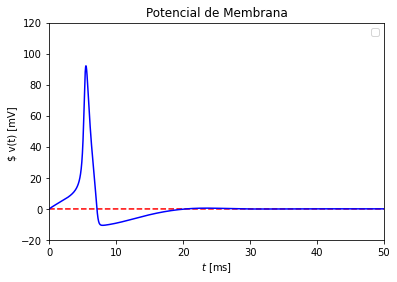
\includegraphics[scale=.4]{figs/potencial_de_membrana.png}
%\vspace{-0.25cm}
\caption{Potencial de membrana con función de corriente constante 0. \label{fig1}}
\end{figure}


Como resultado de la razón de cambio del potencial anterior en los primeros [ms] las fracciones de canales activos de sodio $m(t)$ se estabilizan en aproximadamente por encima de 0. La fracción de canales de Potasio $n(t)$ se estabilizan en aproximadamente 0.3 y la fracción de canales inactivos de sodio $h(t)$ se estabilizan en aproximadamente 0.6. Esto se da para ${t \to \infty}$. fig.~\ref{fig2}. Estos son valores de equilibrio que serán utilizados como valores iniciales en los siguientes experimentos.\\


\begin{figure}[h!]
\centering
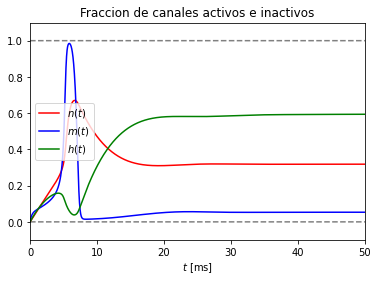
\includegraphics[scale=.4]{figs/fraccion_de_canales_activos_e_inactivos}
%\vspace{-0.25cm}
\caption{Fracción de canales activos e inactivos. \label{fig2}}
\end{figure}


Experimento 2: \textbf{Estímulo débil y estímulo fuerte}. Se utilizo la siguiente función de corriente $i2$.\\
$$
i2(t) = \left\{
\begin{array}{ll}
10 \mu A/cm^2, & t\in [2ms, 2.5ms] \\
30 \mu A/cm^2, & t\in [10ms, 10.5ms] \\
0 \mu A/cm^2, & c.c. \\
\end{array}
\right.
$$

En fig.~\ref{fig3}. se observa que ante el primer estímulo en el intervalo de tiempo [2ms, 2.5ms] la cantidad de corriente inyectada no es suficiente para activar y abrir los canales de sodio por lo cual no se produce un cambio significativo de potencial en la membrana. En cambio para intervalo de tiempo [10ms, 12.5ms], la corriente alcanza el umbral de activación del canal de sodio logrando abrirse dejando pasar los iones de sodio rápidamente lo cual provoca un disparo del potencial. Luego se produce el proceso de repolarización e hiperpolarización  restaurando el sistema a los valores de equilibrio.\\


\begin{figure}[h!]
\centering
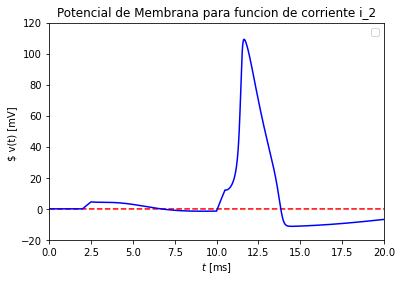
\includegraphics[scale=.4]{figs/potencial_membrana_i_2.png}
%\vspace{-0.25cm}
\caption{Potencial de membrana función i2. \label{fig3}}
\end{figure}

En concreto se observa que la Fracción de $nt$ y $mt$ sube a valores altos entre [0.8, 1] y baja a cerca de  0 para $h(t)$ en el periodo de tiempo [10ms, 12.5ms],
fig.~\ref{fig4}. lo cual indica que en ese periodo de tiempo el flujo de iones puede pasar por la membrana.
Luego del disparo, las fracciones vuelven a valores de equilibrio.
Observar que este modelo inicia en los valores de equilibrio obtenidos en el experimento 1).\\



\begin{figure}[h!]
\centering
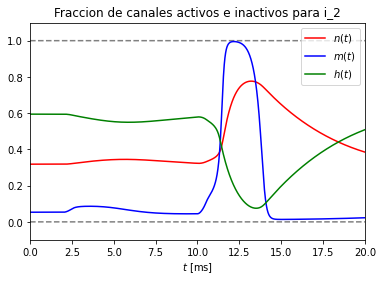
\includegraphics[scale=.4]{figs/fraccion_de_canales_activos_e_inactivos_para_i_2.png}
%\vspace{-0.25cm}
\caption{Fracción de canales activos e inactivos i2. \label{fig4}}
\end{figure}

Experimento 3: \textbf{Ráfaga}. Se utilizo la siguiente función de corriente $i3$ para modelar una rafaga de iones.
$$
i3(t) = \left\{
\begin{array}{ll}
10 \mu A/cm^2, & t\in [5ms,\infty ms) \\
0 \mu A/cm^2, & c.c. \\
\end{array}
\right.
$$

Podemos observar en fig.~\ref{fig5} que después de los  5[ms] se envía constantemente una corriente de 10$uA$. Inmediatamente el potencial de la membrana se dispara por el proceso de despolarización, luego el proceso de despolarización e hiperpolarización llevan  a la membrana a sus nuevos valores de equilibrio. En este tiempo una neurona no puede ser activada nuevamente. Este ciclo se repite desde los nuevos valores de equilibrio y se observa el mismo comportamiento en cada disparo del potencial.\\


\begin{figure}[h!]
\centering
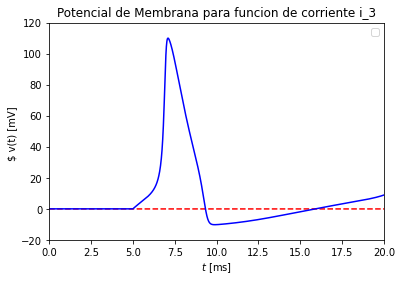
\includegraphics[scale=.4]{figs/potencial_membrana_i_3.png}
%\vspace{-0.25cm}
\caption{Potencial de membrana función i3. \label{fig5}}
\end{figure}


Al igual que en el experimento 2 se observa que las fracciones de canales activos e inactivos inician a partir de los valores de equilibrio.fig.~\ref{fig6}.\\
Aunque en este caso las fracciones son actualizadas en un ciclo infinito donde las fracciones de $nt$ y $mt$ suben y luego vuelven a su valor de equilibrio y $ht$ baja y luego vuelve a su valor de equilibrio. \\

\begin{figure}[h!]
\centering
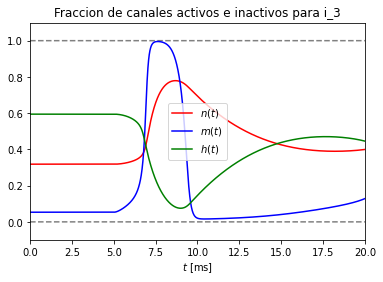
\includegraphics[scale=.4]{figs/fraccion_de_canales_activos_e_inactivos_para_i_3.png}
%\vspace{-0.25cm}
\caption{Fracción de canales activos e inactivos i3. \label{fig6}}
\end{figure}


Experimento 4: \textbf{Período refractario}. Se utilizo la siguiente función de corriente $i4$ para analizar un período refractario.
$$
i4(t) = \left\{
\begin{array}{ll}
10 \mu A/cm^2, & t\in [10ms\, k,10 ms\, k + 2ms], k > 0\\
0 \mu A/cm^2, & c.c. \\
\end{array}
\right.
$$

En este experimento la corriente sigue siendo constantemente 10$uA$, pero no durante todo el tiempo, sino que se envía ese flujo durante intervalos de tiempo espaciados de tal manera que durante los periodos de tiempo que comienzan en [10ms - 12ms], [30ms - 32ms] ...etc, la cantidad de iones recibidos es capaz de activar el potencial. mientras que en los periodos de tiempo [20ms - 22ms], [40ms - 42ms]... etc, la carga de iones no es capaz de activar el potencial. Estos periodos son denominados como periodos refractarios  y se definen como el tiempo en el cual una neurona no puede ser activada nuevamente inmediatamente después de un potencial de acción. En el modelo de Hodgkin y Huxley, se explica por la inactivación temporal de los canales de sodio y la lenta vuelta a la configuración original de los canales de potasio. Ver fig.~\ref{fig7}


\begin{figure}[h!]
\centering
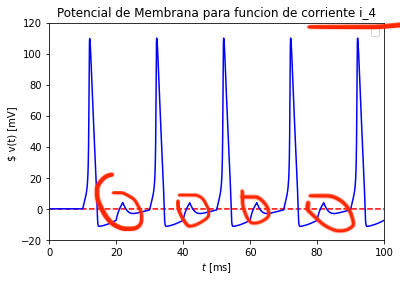
\includegraphics[scale=.4]{figs/potencial_membrana_i_4.png}
%\vspace{-0.25cm}
\caption{Potencial de membrana función i4.\label{fig7}}
\end{figure}



Al igual que en el experimento anterior se observa que las fracciones de canales activos e inactivos inician a partir de los valores de equilibrio.fig.~\ref{fig8}. y luego las fracciones son actualizadas en un ciclo infinito , aunque en este caso la frecuencia es mas baja debido a los periodos refractarios.\\


\begin{figure}[h!]
\centering
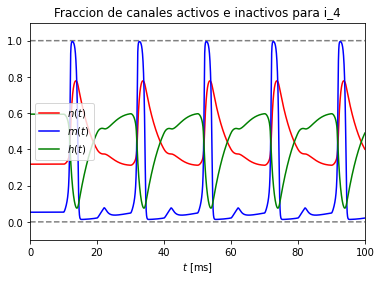
\includegraphics[scale=.4]{figs/fraccion_de_canales_activos_e_inactivos_para_i_4.png}
%\vspace{-0.25cm}
\caption{Fracción de canales activos e inactivos i4. \label{fig8}}
\end{figure}



Experimento 5: \textbf{Exitaciones espontáneas en respuesta al ruido}. Se utilizo la siguiente función de corriente:
$$
i5(t) = \left\{
 50 * \sim i_0 N(0,1)$
\right.
$$

Donde $i_0$  un valor aleatorio obtenido de una distribución normal de media 0 y varianza 1) Por ser un proceso estocástico se integro numéricamente usando el método de Euler.

La corriente en este experimento se modela como un flujo de impulsos aleatorios.

En fig.~\ref{fig9}.


  fig.~\ref{fig10}.
Observar que este modelo inicia en los valores de equilibrio obtenidos en el experimento 1).




\begin{figure}[h!]
\centering
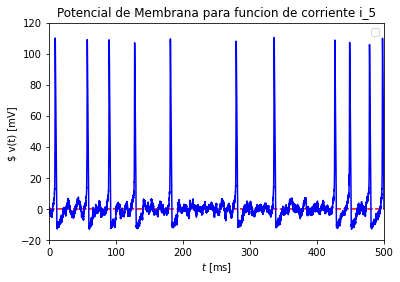
\includegraphics[scale=.4]{figs/potencial_membrana_i_5.png}
%\vspace{-0.25cm}
\caption{Potencial de membrana función i5. \label{fig9}}
\end{figure}





\begin{figure}[h!]
\centering
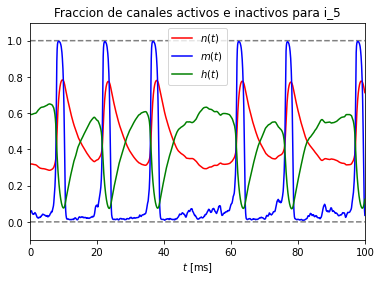
\includegraphics[scale=.4]{figs/fraccion_de_canales_activos_e_inactivos_para_i_5.png}
%\vspace{-0.25cm}
\caption{Fracción de canales activos e inactivos i5. \label{fig10}}
\end{figure}


\section{Conclusiones}

Consideramos que estudiar el modelo de Hodgkin y Huxley es muy propicio para poner en practica los conocimientos adquiridos en cuanto a resolución de sistema de ecuaciones diferenciales. Utilizar herramientas de integración numérica como RK4 implementado en python es también un buen inicio para profundizar el conocimiento en redes neuronales.


% If in two-column mode, this environment will change to single-column
% format so that long equations can be displayed. Use
% sparingly.
%\begin{widetext}
% put long equation here
%\end{widetext}

% figures should be put into the text as floats.
% Use the graphics or graphicx packages (distributed with LaTeX2e)
% and the \includegraphics macro defined in those packages.
% See the LaTeX Graphics Companion by Michel Goosens, Sebastian Rahtz,
% and Frank Mittelbach for instance.
%
% Here is an example of the general form of a figure:
% Fill in the caption in the braces of the \caption{} command. Put the label
% that you will use with \ref{} command in the braces of the \label{} command.
% Use the figure* environment if the figure should span across the
% entire page. There is no need to do explicit centering.

% \begin{figure}
% \includegraphics{}%
% \caption{\label{}}
% \end{figure}

% Surround figure environment with turnpage environment for landscape
% figure
% \begin{turnpage}
% \begin{figure}
% \includegraphics{}%
% \caption{\label{}}
% \end{figure}
% \end{turnpage}

% tables should appear as floats within the text
%
% Here is an example of the general form of a table:
% Fill in the caption in the braces of the \caption{} command. Put the label
% that you will use with \ref{} command in the braces of the \label{} command.
% Insert the column specifiers (l, r, c, d, etc.) in the empty braces of the
% \begin{tabular}{} command.
% The ruledtabular enviroment adds doubled rules to table and sets a
% reasonable default table settings.
% Use the table* environment to get a full-width table in two-column
% Add \usepackage{longtable} and the longtable (or longtable*}
% environment for nicely formatted long tables. Or use the the [H]
% placement option to break a long table (with less control than
% in longtable).
% \begin{table}%[H] add [H] placement to break table across pages
% \caption{\label{}}
% \begin{ruledtabular}
% \begin{tabular}{}
% Lines of table here ending with \\
% \end{tabular}
% \end{ruledtabular}
% \end{table}

% Surround table environment with turnpage environment for landscape
% table
% \begin{turnpage}
% \begin{table}
% \caption{\label{}}
% \begin{ruledtabular}
% \begin{tabular}{}
% \end{tabular}
% \end{ruledtabular}
% \end{table}
% \end{turnpage}

%\section{Aknowledgments}
\section{Agradecimientos}

\begin{acknowledgments}
a FaMAF, siempre FaMAF y a la educación publica.
\end{acknowledgments}
% Create the reference section using BibTeX:
\bibliography{ref}

% Specify following sections are appendices. Use \appendix* if there
% only one appendix.

\onecolumngrid

\appendix


\end{document}
%
% ****** End of file apstemplate.tex ******
